\chapter{Introduction and Background}
\label{ch: intro}

\graphicspath{{Figures/Intro/}{./}} 

In the situation when a large amount of data comes like a flow, data analysts might be interested in the how is the data distributed, or in other words, where are the densely and sparse parts of the distribution. For example, the managers of an online shopping system might be interested in the distribution of customers' age of an online sales event. As they want to find the majority of age groups for a more efficient advertisement, the question of the distribution is "what is the age diving points of the youngest 10\% and the oldest 10\%".  On one hand, the most updated distribution analysis is expected for a rapid adaptation, while on the other hand there is limited storage for the large amount of incoming data. In this paper, we explore this problem as a quantile estimation problem on data streams, and try to find space-efficient and computationally cheap solutions using the stochastic gradient descent method.

\section{Quantiles}
\label{sec: intro_quant}
Quantiles are the cutting points of a statistical distribution by its ranking. Specifically, the $\tau$-quantile is the cutting point that divides the distribution by probability $\tau$. Let $\tau$-q denote the $\tau$-quantile. For example, a $0.5$-q is the median of a distribution, such that there is a $50\%$ probability that a random sample is smaller than it. Generally, the value of a quantile can be achieved by mathematical approaches when the expression of the distribution is given. 
The quantiles are an important statistical feature of distributions for their values roughly reflects the density of the distribution.
For example, Fig \ref{fig: quant_example} shows samples from a Gaussian distribution and is annotated with two intervals [$0.5$-q, $0.9$-q] and [$0.9$-q, $0.99$-q]. The values of the intervals are similar, but the former contains 40\% data and the latter contains only 9\% data. Without any other information, this alone leads to the implication that the distribution is denser in the former interval than the latter.

\begin{figure*}[h!]
    \centering
	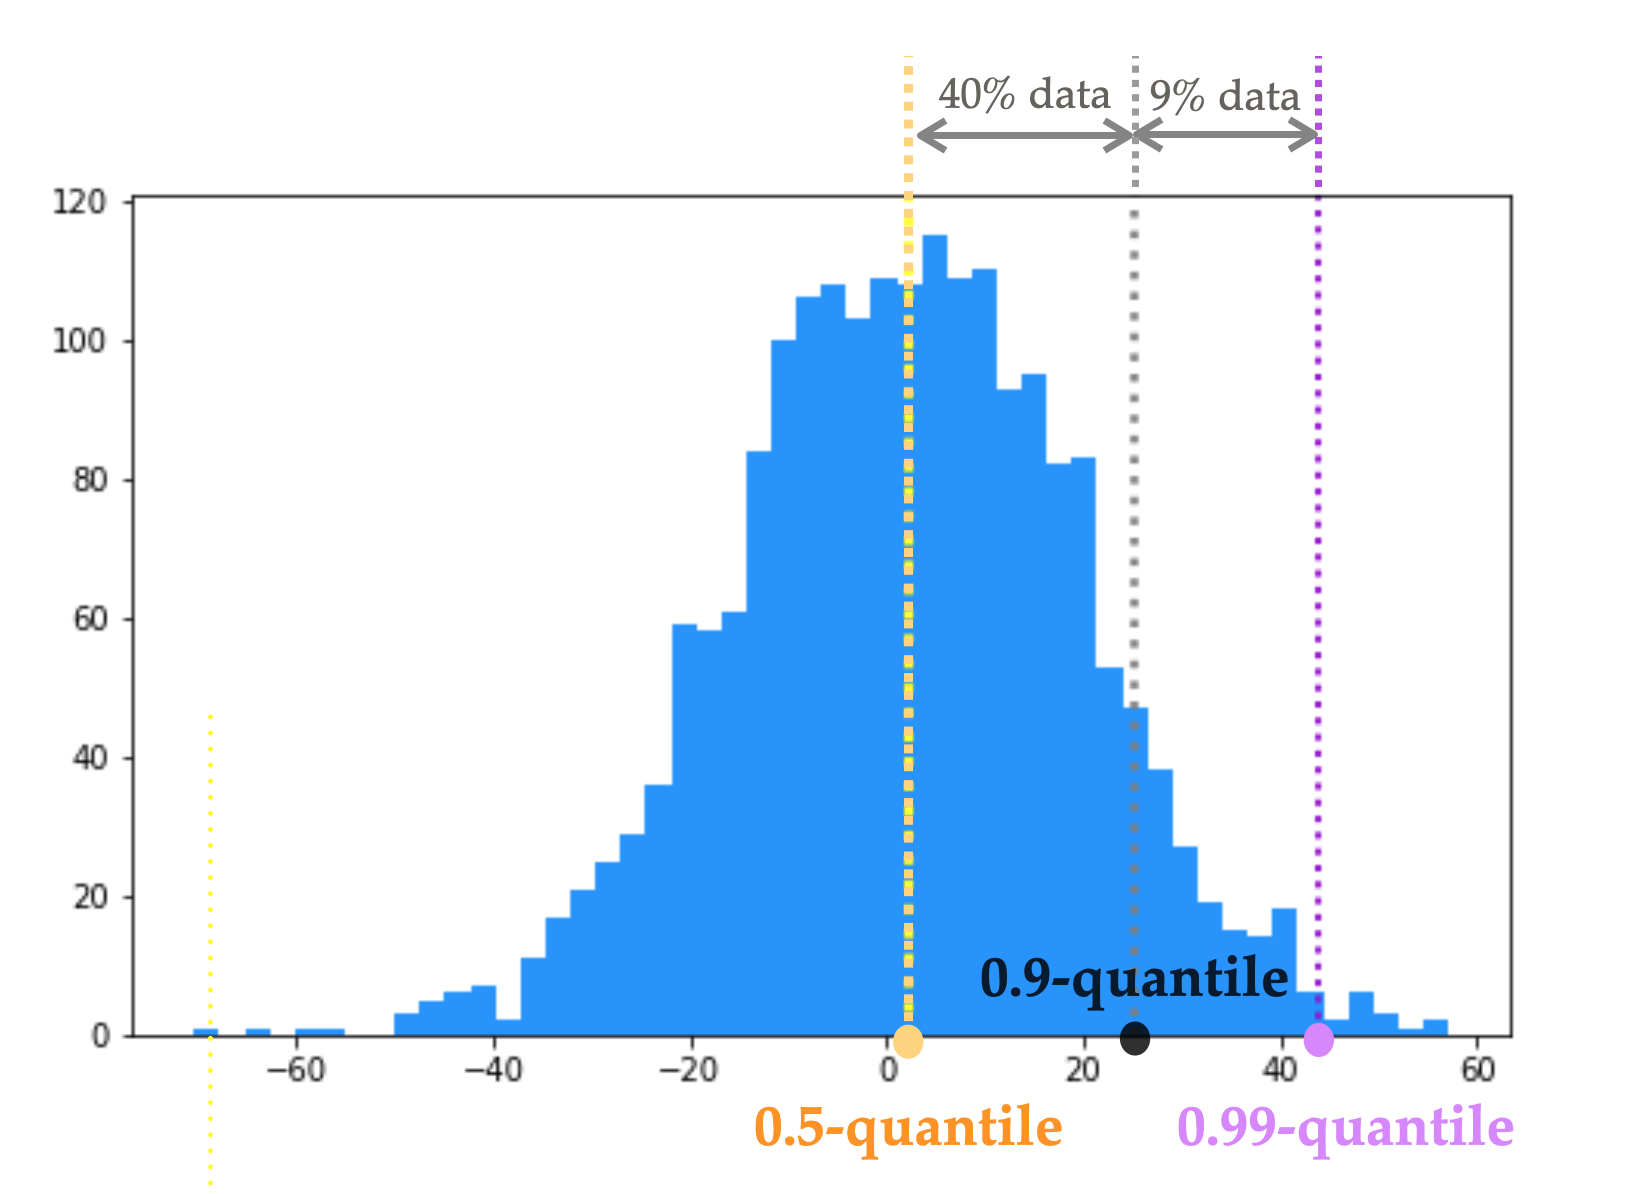
\includegraphics[width=0.6\columnwidth]{quant_example.png}
    \caption{Quantiles (0.5-q, 0.9-q and 0.99-q) of a dataset containing 2000 random samples from a Gaussian distribution (mean = 2, standard deviation = 18)}
    \label{fig: quant_example}
\end{figure*}

As shown in the example of Fig \ref{fig: quant_example}, the concept of quantiles are also applied in datasets as well as probability distributions. Similarly, the quantile for a finite dataset is the point which divides the dataset by probability $\tau$. However, since the dataset is discrete, the value of a $\tau$-q is ambiguous. For example, for dataset [$1,2,3,4$], both 2.01 and 2.99 can be considered as a valid value of $0.5$-q. Among various methods of dataset quantile estimations, we apply the one currently used by the \textit{Python 3} language. For a size $N$ dataset $X = \{x_1, ..., x_N\}$ , the method first finds the ranking index of the quantile $h = (N-1)\tau + 1$. If $h$ is not an integer, the estimated quantile is computed by linear interpolation between the two data points at ranking positions surround $h$
\begin{equation}
    \tau \text{-q}_{batch} = x_{\lfloor h\rfloor}+(h-\lfloor h\rfloor)\left(x_{\lfloor h\rfloor+1}-x_{\lfloor h\rfloor}\right)
\end{equation}
where $\lfloor h\rfloor$ is the greatest integer less than or equal to $h$. The computation result $\tau \text{-q}_{batch}$ is called a \textit{batch quantile}, since it comes from a batch of samples of a distribution.
\\\\
Note that although computing the quantiles of a sample estimates the quantiles of the associated distribution, this is not \"quantile estimation\" as it is referred to in this paper. Here the batch quantiles are regarded as computed quantiles, as a comparison of \textit{true quantiles} which are the real quantiles of the original probability distribution. The estimation of quantiles is introduced in the following part.

% Batch algorithm/True quantile: the naive sorting

\section{Data streams and quantile estimation}
\label{sec: intro_quant_est}

A \textit{Data stream} is a large source of data where data is created in sequence over a period of time. In contrast with datasets, data points are not instantly available all at a time, and that the size of the sample grows over time. Data streams are commonly seen in areas like network monitoring, data mining, financial trading systems, etc. Similarly to normal datasets, the value of quantiles is important for data analysis of data streams. Finding the quantiles of a data stream is the initial aim of this paper.

A trivial solution to find quantiles of data streams is to sort the entire data stream when the last data point arrives, and then compute the batch quantiles of the sorted dataset.  In cases when the size of the data stream is unknown, at the arrival of each data point, the batch quantiles are computed again so the quantile values get updated. The method of repeatedly sorting and computing batch quantiles is called the \textit{batch algorithm}. Due to the large size of the data streams, the batch algorithm for quantile computation is too expensive in both storage and computation to be a feasible solution for most computer systems.

Faced with the storage and computation problem, algorithms of \textit{quantile estimation} on data streams have been proposed. The quantile estimation algorithms do not store the entire data streams, and the algorithms return estimated quantiles that are close to the batch quantiles. Some quantile estimation algorithms are described in the literature review chapter. Although these algorithms use significantly less memory than the batch algorithm, most require a growing space complexity (i.e., correlated with size $N$). In this paper we investigate the space-efficient algorithms that use constant memory units for data streams of any size. Specifically, we focus on the machine learning method \textit{stochastic gradient descent} (SGD) for quantile estimation. 

\section{Stochastic gradient descent(SGD) for quantile estimation}
\label{sec: intro_GD_SGD}

\textit{Gradient descent} is a convex optimization algorithm that is commonly used in machine learning for loss function minimization. Gradient descent takes the entire dataset as the input, and by iteratively moving in the opposite direction of the gradient, it reaches the local minimum. Such method can also be used in quantile estimation if the entire dataset is available all at the same time.

\textit{Stochastic gradient descent (SGD)}, on the other hand, is the "online learning" version of gradient descent that updates iteratively when each new data point comes. For each data point, SGD steps in the opposite direction of the gradient computed from that data point. In this way, SGD updates using one data point at a time, rather than the whole dataset.
Fig \ref{fig: SGD_quant} shows how SGD is used to estimate quantiles on the same dataset of 2000 Gaussian distribution samples from Fig 1. It is shown in the figure that the SGD result fluctuates around the empirical quantile value, indicating SGD is a possible approach for quantile estimation.

\begin{figure*}[h!]
    % \centering
	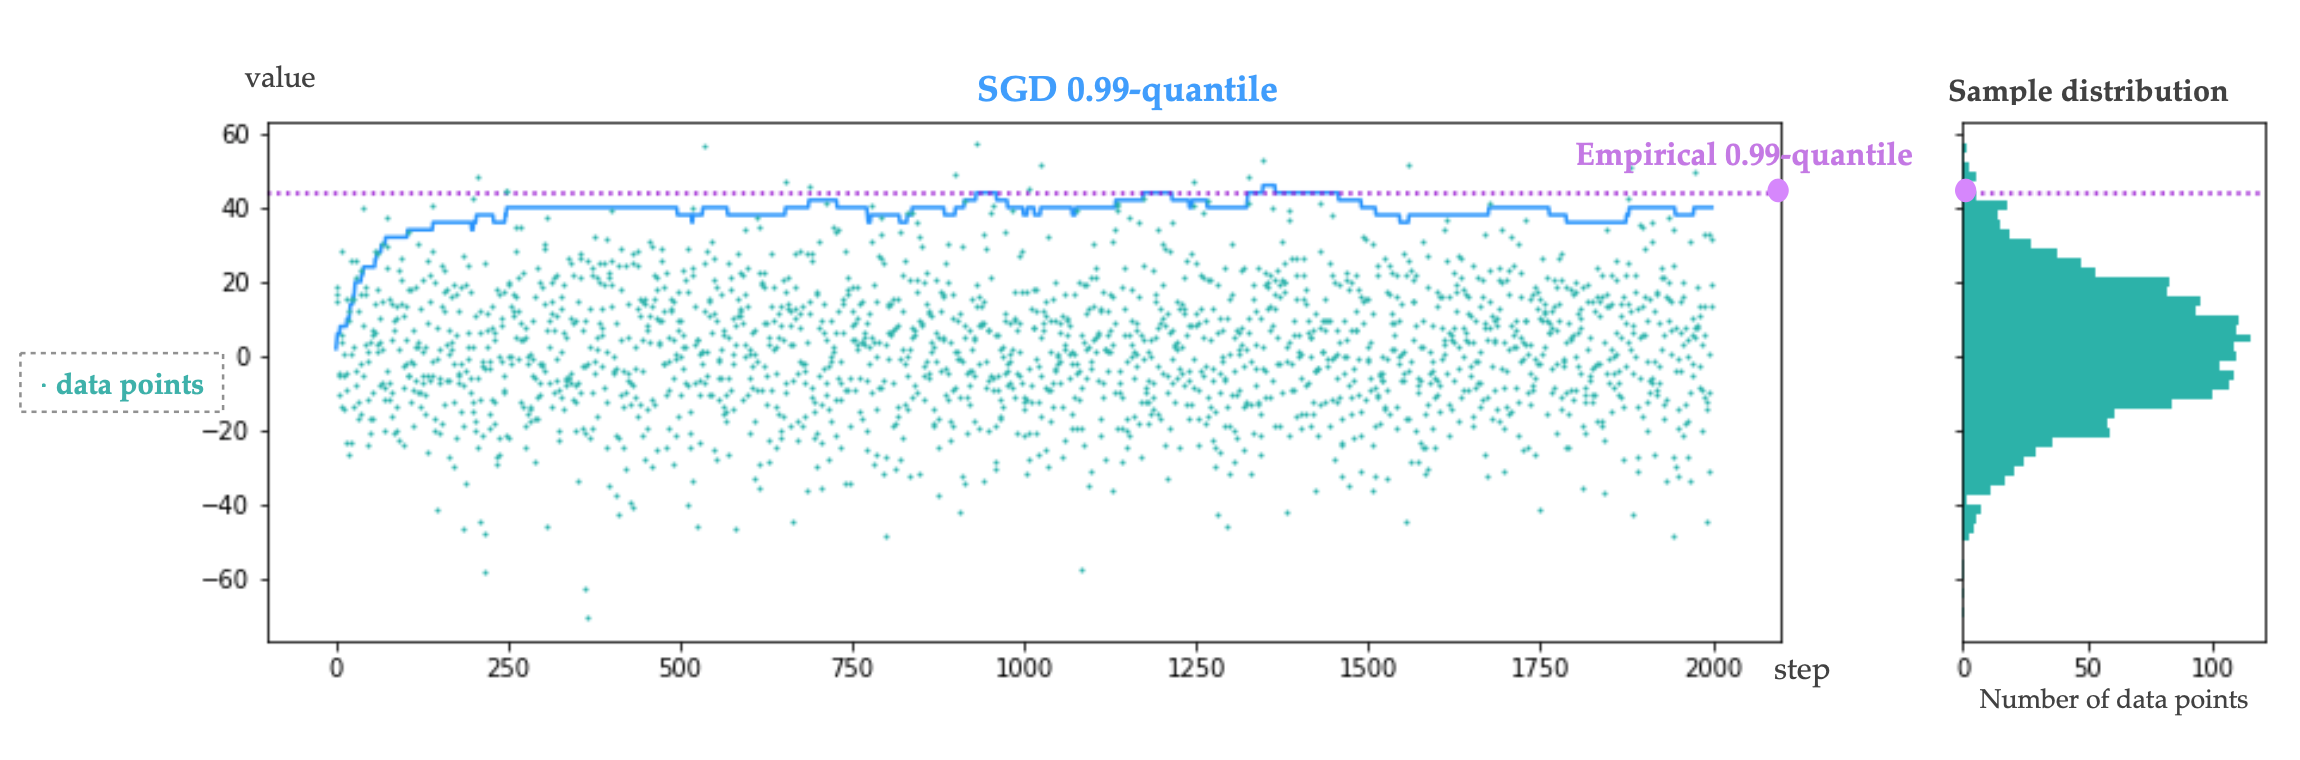
\includegraphics[width=1\columnwidth]{SGD_gaussian.png}
    \caption{SGD quantile estimation of the $0.99$-q for a dataset of 2000 samples from a Gaussian distribution. The left graph is a combination of incoming data points and the SGD steps, and each step of SGD is triggered by a new coming data point. The blue line shows how the SGD result is updated on the arrival of a data point (sea-green), and straight line (violet) represents the empirical value of $0.99$-q. On the right side, the density of the bell-shaped dataset is shown in a histogram.}
    \label{fig: SGD_quant}
\end{figure*}


\section{Background}

In this chapter, the essential background knowledge assumed throughout the rest of this thesis is defined. Subsection~\ref{subsec: sgd}introduces Stochastic Gradient Descent (SGD), which is a convex optimisation approach commonly found in machine learning, and subsection~\ref{subsec: quant} provides a definition for quantiles.
Stochastic gradient descent (SGD) is a convex optimization approach commonly applied in machine learning, and quantiles are the dividing points of a distribution or a dataset.

    \subsection{Gradient descent and stochastic gradient descent}
    \label{subsec: sgd}
    Stochastic gradient descent is an optimization algorithm developed from gradient descent. 
    \marginpar{References to be added here}
    Gradient descent was introduced by \textcolor{blue}{someone}, and is commonly used in \textcolor{blue}{something}

    \subsubsection{Gradient Descent}
        For convex optimization problems, gradient descent is a first-order optimization algorithm 
        to find the local minimum of a function.
        \\\\
        To solve the minimization problem 
        \begin{equation}
            % E
            \min_{\x} L(\x) 
        \end{equation} 
        
        where $L : \R^d \to \R$ is convex, differentiable and its gradient is Lipschitz continuous with constant
        $L > 0$.
        \\\\
        Geometrically, the gradient $\nabla L(\x_0)$ points to the direction of the steepest ascent on $L(\cdot)$ 
        from the point $\x_0$. 
        By taking a small step in the direction of the negative gradient, the function value is decreased in the 
        direction of the steepest descent. That is,
        \begin{equation}
            \x_1  = \x_0 - \alpha \nabla L(\x_0)
        \end{equation}
        for a small enough step size $\alpha \in \R_{+}$, then $L(\x_1) \leq L(\x_0)$. 
        That means, compared with $L(\x_0)$, $L(\x_1)$ is closer to the local minimum.
        \\\\
        With this observation comes the idea of gradient descent: an iterative "tour" on $L(\cdot)$ from a point towards the 
        local minimum by following small steps of negative gradient. 
        Let $\x_0$ be the guess of a starting point, then if
        % \marginpar{notation k should be i}
        \begin{equation}
            \x_{i+1} = \x_{i} - \alpha_i \nabla L(\x_i), i \geq 0
        \end{equation}
        
        
        Then we have $ L(\x_0) \geq L(\x_1) \geq L(\x_2) \geq \cdots$ where $\alpha_i$ is a suitable step size for iteration $i$. The convergence rate of the 
        sequence $(\x_n)$ with certain step size settings is linear in terms of the number of iterations.

        The objective function $L(\cdot)$ can be written as a sum of differentiable functions:%
        \begin{equation}
            L(\x) =\frac{1}{N} \sum_{n=1}^{N} \ell_n (\x)
        \end{equation}

        where the \textit{summand function} $\ell_n$ is usually the loss function of the $n$th observation among
        $N$ data points.
        \\\\
        Applying the gradient descent formula, $\x$ is updated according to%
        %
        \begin{equation}
           \x_{i+1} = \x_{i} -\alpha_i \nabla L(\x_i) = \x_{i} -\alpha_i \frac{1}{N}\sum_{n=1}^{N} \nabla \ell_n(\x_i) 
           \label{eq: background_gd_summand}
        \end{equation}

        From formula~\ref{eq: background_gd_summand}, it is clear that gradient descent requires access to all the data points to compute the movement direction, which is infeasible for a data stream.


    \subsubsection{Stochastic Gradient Descent (SGD)}
        Stochastic gradient descent was \textcolor{blue}{introduced by who because blabla, and commonly used bla}
        It is the choice for data streams, because the computation of the movement direction relies only on the most recent data point.
        It can be considered as a stochastic approximation of gradient descent optimization.
        \\\\
        The calculation of $\sum_{n=1}^{N} \nabla \ell_n(\x_i)$ can be
        expensive, especially when the amount of summand functions is huge, or when the individual gradients are hard to
        compute.
        To reduce the calculation, an estimation of the true gradient of $L(\x)$ is taken: 
        the true gradient $\frac{1}{N} \sum_{n=1}^{N} \nabla \ell_n(\x_i)$ is replaced by the gradient with respect to the $m$th observation, $\nabla \ell_m(\x_i)$. 
        So the update of the parameter $\x$ becomes%
        \begin{equation}
            \x_{i+1} = \x_i - \alpha_i \nabla \ell_m(\x_i)
            \label{eq: intro_SGD}
        \end{equation}
        
        Generally, each time $m$ is randomly selected from $N$. In this paper, we use $m = i$ for quantile estimation on data streams.

\subsubsection{Limitations}
\marginpar{Not sure how I should mention this non-differentiable issue}
Since each SGD update requires only a single data point instead of the entire dataset, it becomes a great alternative for quantile estimation.
However, neither GD nor SGD can handle non-differentiable functions. This is an issue for the quantile estimation loss function in the following chapter.
Furthermore, while the computation per update is decreased $N$ times, the tradeoff lies in the convergence rate. SGD does not enjoy the same linear convergence rate as gradient descent. Both of these issues are discussed in chapter~\ref{ch: stepsize_adaptation}.


\subsection{Quantile}
\label{subsec: quant}

In statistics, quantiles are the points that divide a probability distribution into even intervals.
The $q$-quantiles ($q \in \{2,3,4,...\}$) is a set of quantile points which divides the distribution into $q$ intervals each with the same probability mass.
For example, the $2$-quantile has only one quantile point, which is the middle point of the distribution
and it divides the distribution into two even parts. This $2$-quantile point is called the median.
        \\\\
    \textbf{Definition with $q$-quantile notation} \\
    Generally, the $q$-quantiles have $q-1$ quantile points, and the $k$th quantile point for a 
    distribution $X$ is the data value such that%
    %
    \begin{equation}
        Pr(X \leq x) \geq \frac{k}{q}
    \end{equation}
    
    and%
    %
    \begin{equation}
        Pr(X \geq x) \geq 1 - \frac{k}{q}
    \end{equation}
    where $x \in X$.
    \\\\
    \textbf{Definition with notation $\tau$}\\
    Since $k < q$, we have $0 < \frac{k}{q} < 1$ for all ($k$,$q$) pairs. For $k, q \in \mathbb{N}^+$ we can define a quantile for any rational number in the interval $(0,1)$. For a quantile probability $\tau$, we use the notation $\tau$-quantile ($0 < \tau < 1$) for a quantile value in the distribution $X$ that satisfies%
    %
    \begin{equation}
        Pr(X \leq x) \geq \tau
    \end{equation}
    
    and%
    %
    \begin{equation}
        Pr(X \geq x) \geq 1 - \tau
    \end{equation}
    where $x \in X$.



\section{Thesis overview}
\label{sec: intro_overview}

This thesis aims to thoroughly answer the following question:
\begin{quote}
\emph{Can SGD be used for effective quantile estimation?}
\end{quote}

In investigating the above research question, this thesis includes the following contributions:
\begin{enumerate}
    \item Proposal of the SGD algorithm for quantile estimation which implements the SGD approach.
    \item SGD algorithm performance comparison with the state-of-the-art Frugal1U.
    \item Identification of some contributing factors on SGD performance.
    \item Improved SGD methods with quicker convergence rate to the true quantile value.
    \marginpar{This is not counted as a contribution I think?}
    \item Experiments on other people's methods that simultaneously estimate different quantiles at the same time, which is a potential improvement direction for SGD too.
\end{enumerate}

In the final part of the introduction, we give a brief tour of the material in this paper. The main focus of the paper is to explore how stochastic gradient descent method can be used for quantile estimation on data streams.
In chapter \ref{ch: literature_review}, a very brief discussion of quantile estimation algorithms is presented, with a special mention for space-efficient algorithms (e.g., SGD-like methods). 
Chapter \ref{ch: algo_equal} compares the SGD methods with the \textit{Frugal1U} algorithm\cite{maFrugalStreamingEstimating2014}, showing how the two similar methods are "equivalent" to some extent.
Chapter \ref{ch: sgd_exp} which presents experiments to illustrate the relationship between setting for SGD and its performance.
Next, chapter \ref{ch: stepsize_adaptation} and \ref{ch: multi_quant} explore the two extensions of the vanilla SGD algorithm: the step size adaptation of SGD and the simultaneous multi-quantile estimation. Finally, the work of the paper is summed up in the conclusion chapter \ref{ch: conclusion}.
\\\\
Fig \ref{fig: structure} is the layout of the contents of the paper.

\begin{figure*}[h!]
    \centering
	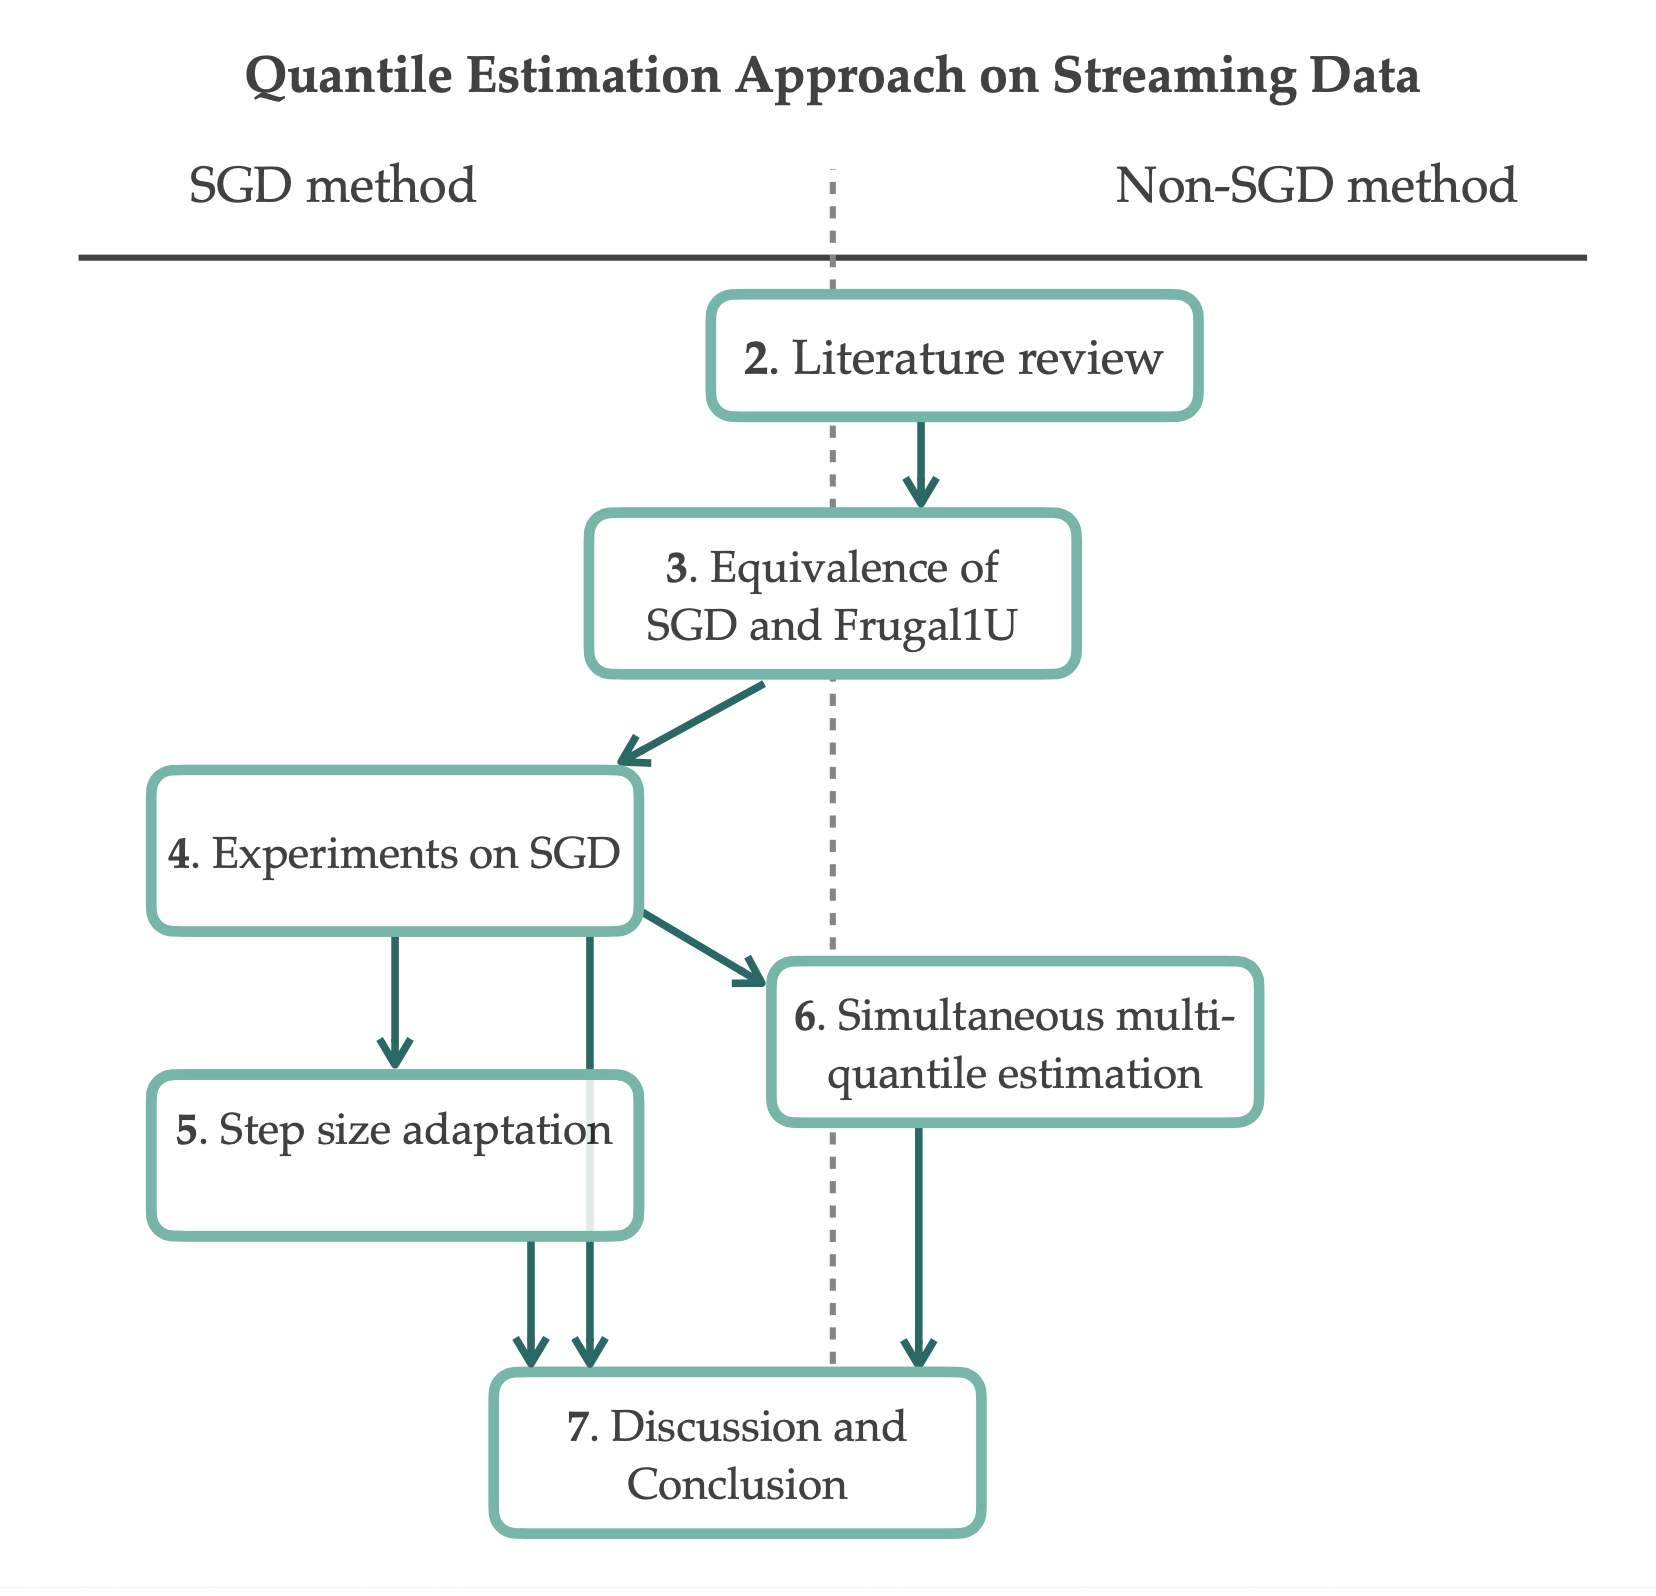
\includegraphics[width=0.8\columnwidth]{structure.png}
    \caption{The relationship between topics covered in the thesis. Topics are roughly positioned along the top-bottom axis depending on where they are more close to SGD methods (left) or non-SGD methods (right). The arrows between the chapters represent are connected according to dependence.}
    \label{fig: structure}
\end{figure*}

\marginpar{My contributions to be added here}